% !TeX spellcheck=en_GB
\section{Theoretical part - formulation and lower bounds}
Given a complete directed graph $G = (V,E),c$ with $|V| = n$ where $c_{ij}$ is the cost of the edge from vertex $i$ to vertex $j$, the asymmetric travelling salesman problem is to find a minimum cost Hamiltonian tour of G.

The subtour integer linear programming formulation for the travelling salesman problem as follows:

\[ 
x_{ij} =
\left \{
  \begin{tabular}{cc}
  1, & if edge (i,j) is included\\
  0, & otherwise 
  \end{tabular}
\right .
\]

\begin{alignat*}{4}
\text{max: }    & \sum_{i,j \in V} c_{ij} x_{ij}\\
\text{s.t }     & \sum_{i \in V, i \neq j} x_{ij} = 1  && \text{ for } j \in V && (1)\\
                & \sum_{j \in V, j \neq i} x_{ij} = 1  && \text{ for } i \in V && (2)\\
                & \sum_{i,j \in S} x_{ij} \leq |S| - 1 && \text{ for } S \subset V \text{ such that } 2 \leq |S| \leq n - 2 \quad && (3)\\
                & x_{ij} \in \{0,1\} && && (4)
\end{alignat*}

\subsection{} % 1.1
In this proof we do not need to take into consideration the objective function or the cost of a Hamiltonian tour since these do not affect the feasibility of a solution.

First we prove that any feasible solution will satisfy the above constraints. Constraint $(1)$ requires that all vertices in $G$ must have exactly one incoming edge. All vertices in a Hamiltonian tour will per definition satisfy this. Constraint $(2)$ requires that all vertices in $G$ must have exactly one outgoing edge. All vertices in a Hamiltonian tour will per definition satisfy this. These constraints in combination requires that there can only exist cycles in $G$ and that every vertex is part of exactly one cycle. A Hamiltonian tour is the special case of graphs with cycles where only one cycle exists which visits every vertex of the graph, hence it naturally satisfies the constraints. Constraint $(3)$ requires a solution to, for all proper subsets $S $ of $V$ such that $2 \leq |S| \leq |V| - 2$ have less edges than vertices. Note that a cycle visiting $k$ vertices must have $k$ edges. Therefore the constraint requires that no cycles exist in all graphs induced by all proper subsets of $V$. For all graphs induced by all proper subsets of the vertices of a Hamiltonian tour there exists no cycles. Therefore any feasible solution also satisfies this constraint. Constraint $(4)$ is naturally satisfied since a feasible solution does not have a concept of partially traversing edges. This concludes the first part of the proof.

Now we need to prove that any solution satisfying the constraints is also a feasible solution. A Hamiltonian tour is a single cycle which enters every vertex of the graph exactly once. For the sake of proof by contradiction we assume there exists a solution $H$ that satisfies the constraints but is not a feasible solution, that is, it is not a Hamiltonian tour. First we assume that $H$ does not form a cycle in $G$. This implies that there exists a vertex $v$ which has in or out-degree not equal to $1$. But this contradicts constraints $(1)$ or $(2)$ and hence no such $H$ can exist. Now we assume that there exists a vertex $v$ which is not part of a cycle in $H$. This implies that $v$ has an in or out-degree equal to $0$ which contradicts constraints $(1)$ or $(2)$. We now assume that $H$ consist of multiple cycles. This implies that for some proper subset of $H$ the number of vertices covered by the subset of edges is equal to the number of edges. But this contradicts constraint $(3)$. We have therefore shown that any solution satisfying the constraints must be a single cycle which enters every vertex of $G$ exactly once, that is, a Hamiltonian tour of $G$ which is a feasible solution to the Travelling Salesman Problem. This concludes the proof.

\subsection{}  % 1.2
First we calculate the number of subsets $S \subset V \text{ such that } |S| \leq n - 2$. This number corresponds to counting every subset of size up $n-2$ out of $n$, minus the number of subsets of size $1$ which naturally is $n$. This gives the following size: $\frac{n!}{(n-2)! (n - (n-2))!}-n = \frac{n!}{2 (n-2)!}-n$. Hence there are exponentially many constraints of this type. 


\subsection{} % 1.3

The compact formulation is as follows:

\begin{alignat}{3}
	\text{max: }    & \sum_{i,j \in V} c_{ij} x_{ij}\\
	\text{s.t }     & \sum_{i \in V, i \neq j} x_{ij} = 1  && \text{ for } j \in V\\
	& \sum_{j \in V, j \neq i} x_{ij} = 1  && \text{ for } i \in V\\
	& t_j \geq t_i + 1-n(1-x_{ij})  && \text{ for } i \in V, j \in V \setminus \{1\}\\
	& x_{ij} \in \{0,1\} \\
	& t_i \in \mathbb{R}_+ 
\end{alignat}

Constraints $(7)$ runs over two variables, $i,j$ which can have $n$ and $n-1$ different values respectively. Therefore there are $n(n-1) = n^2-n$ many constraints. Hence there are polynomially many constraints of this type.

\subsection{} % 1.4
The constraints of the sub tour formulation might provide for a better branching decision in a branch and bound scenario and further more the constraints might be more restricting to integer solutions, so branch and cut might not be as necessary.

\subsection{} % 1.5
Consider the minimum cost Hamiltonian tour $H$, it goes through vertex $1$. Vertex $1$ has exactly two edges incident to it in $H$. If we remove one of them, creating a path, the solution is a tree with $1$ as root covering every vertex in $V$. Since the lower bound algorithm finds a minimum cost tree, the cost will be lower than or equal to the cost of the tree of $H$. If the removed edge from $H$ is the edge with the lowest cost connecting vertex $1$ to the tree, then the lower bound algorithm would also pick it. If there exists an edge with lower cost than the removed edge connecting vertex $1$ to the tree, then the algorithm will pick the cheaper and therefore still  provide a lower bound to $H$. This concludes the proof.

\section{Implementation part - branch-and-bound}
\subsection{}
We propose a simple heuristic, which while not necessarily can be used to generate feasible solutions, provides an upper bound to the $TSP$ as required. For each vertex of the graph pick the most expensive incident edge. If the edge is already in the upper bound solution pick the second most expensive. 

This is clearly an upper bound as the optimal solution will have to visit each vertex $i$ via an edge $e$ which will have lower than or equal to cost than the most expensive edge going to $i$. This can trivially be calculated in $\mathcal{O}(n+m)$ time, with the right data structure, where $n$ is the number of vertices and $m$ is the number of edges. This heuristic will work on any graph.

Using this heuristic the upper bound for instance $1$ is computed to $31.084$.

\subsection{}
Instance 1:

\newpar \textbf{Solved by branch-and-bound}\\
Path-length: 8,649\\
213750 nodes generated\\
Took 1834,46ms

\newpar \textbf{Solved by CPLEX using formulation from assignment 1.1}\\
Path-length: 8.648571749039572\\
Took 310,01ms

\newpar \textbf{Solved by CPLEX using the formulation from assignment 1.3}\\
Path-length: 8.648571749039572\\
Took 348,38ms

\begin{figure}[H]
	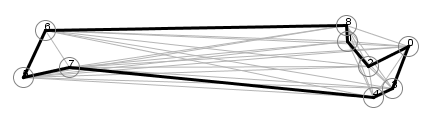
\includegraphics[width=.9\textwidth]{figures/Instance1Solution.png}
	\caption{Solution to instance 1}
	\label{solution:1}
\end{figure}

\noindent Instance 2:

\newpar \textbf{Solved by branch-and-bound}\\
Path-length: 19,030\\
1539573 nodes generated\\
Took 13099,38ms

\newpar \textbf{Not solved by CPLEX using formulation from assignment 1.1}\\
Too many subsets to build the CPLEX-instance.

\newpar \textbf{Solved by CPLEX using the formulation from assignment 1.3}\\
Path-length: 19.02956846604248\\
Took 221,01ms

\begin{figure}[H]
	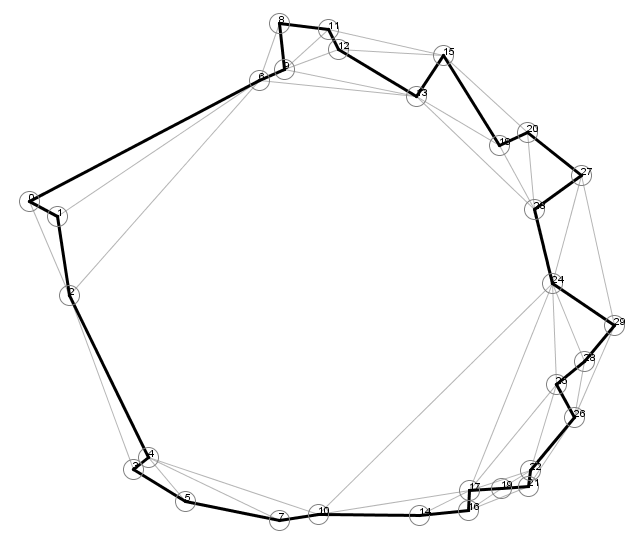
\includegraphics[width=.9\textwidth]{figures/Instance2Solution.png}
	\caption{Solution to instance 2}
	\label{solution:2}
\end{figure}

\newpar Instance 3:

\newpar \textbf{Not solved by branch-and-bound due to time limits.}

\newpar \textbf{Not solved by CPLEX using formulation from assignment 1.1}\\
Too many subsets to be generated.

\newpar \textbf{Solved by CPLEX using the formulation from assignment 1.3}\\
Path-length: 26.544022448704812\\
Took 1370,51ms

\begin{figure}[H]
	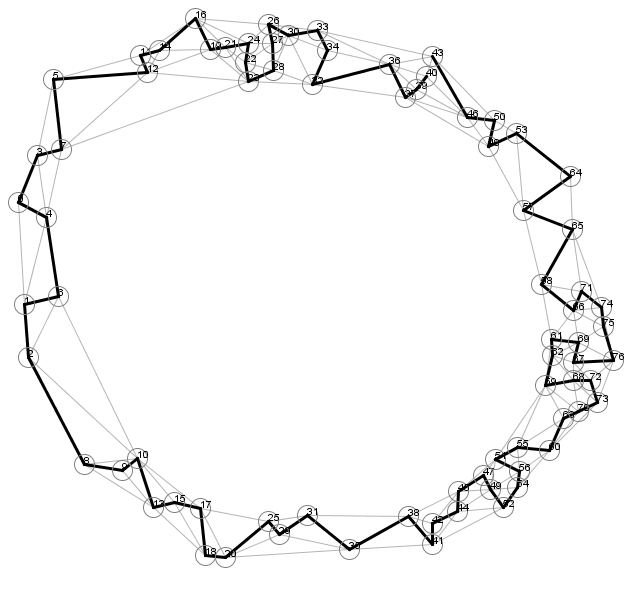
\includegraphics[width=.9\textwidth]{figures/Instance3Solution.png}
	\caption{Solution to instance 3}
	\label{solution:3}
\end{figure}


\subsection{}